% Document class
\documentclass[titlepage]{report}

% Packages
\usepackage{lipsum,eurosym,enumitem,multicol,hyperref,geometry,graphicx,float,listings}
\usepackage[utf8]{inputenc}
\usepackage[T1]{fontenc}
\usepackage[dvipsnames]{xcolor}
\usepackage[english]{babel}
\usepackage{subfig}
\usepackage{float}
\usepackage{listings}
\usepackage{qrcode}

\setcounter{tocdepth}{3}
\setcounter{secnumdepth}{3}

\DeclareFixedFont{\ttb}{T1}{txtt}{bx}{n}{9} % for bold
\DeclareFixedFont{\ttm}{T1}{txtt}{m}{n}{9}  % for normal

% Custom colors
\usepackage{color}
\definecolor{deepblue}{rgb}{0,0,0.5}
\definecolor{deepred}{rgb}{0.6,0,0}
\definecolor{deepgreen}{rgb}{0,0.5,0}
\newcommand\pythonstyle{\lstset{
language=Python,
basicstyle=\ttm,
keywordstyle=\ttb\color{deepblue},
emph={MyClass,__init__},          % Custom highlighting
emphstyle=\ttb\color{deepred},    % Custom highlighting style
stringstyle=\color{deepgreen},
frame=false,                         % Any extra options here
showstringspaces=false
}}
\lstnewenvironment{python}[1][]
{
\pythonstyle
\lstset{#1}
}
{}


% Document geometry
\geometry{paper=a4paper,textwidth=16cm}

% Premiere pages
\begin{document}

\pagenumbering{arabic}
    \begin{center}

    \begin{figure}[htbp]
        \centering
        
\includegraphics[width=0.5\columnwidth]{Logo.svg.png}
    \end{figure}
    \vspace{0.5cm}

    \vspace{1.5cm}
    \Huge{\bfseries APU } \\
    \vspace{3cm}
    \Huge{\bfseries Fantome Escape} \\
    \Huge{\bfseries Projet Programmation Python 2023}\\
    \vspace{3cm}
    \huge{Lucien PIAT} 
    \huge{Sara SPIELER} \\
    \vspace{3cm}
    
    \Large Superviseurs:\\
    \vspace{0.5cm}
    \begin{minipage}{0.30\textwidth}
     \centering
    \Large{M. Beurton-Aimar}
    \end{minipage} 
    \end{center}
\thispagestyle{empty} 


    
% Table of contents
\newpage
\tableofcontents
\thispagestyle{empty} 

%Debut du sujet 
\newpage
\pagenumbering{arabic} 

\section{Introduction}
\hspace*{0.5cm}Afin de nous familiariser avec l'outil de programmation Python, nous a été donné à la fin du semestre un projet à coder avec ce dernier. Il s'intitule Fantôme Escape mais nous l'appelons formellement Casper. Le code que nous devons produire affichera un jeu dans le terminal ou l'objectif est d'emmener Casper le fantôme de la réception d'un château au paradis.\\
\hspace*{0.5cm}Dans ce rapport, nous décrirons, nos diverses idées pour implémenter le jeu, nos faux pas lors de sa création, et finalement, les diverses fonctions et le programme principal que nous avons retenues. 


\section{Analyse du sujet}
\subsection{Division du sujet}
\hspace*{0.5cm} Le sujet peut être divisé en 3 parties, l'affichage du plateau de jeu, le déplacement du joueur, et l'action des différents méchants qu'on peut trouver dans le jeu.\\
\hspace*{0.5cm}Au niveau de l'affichage plusieurs éléments méritent une attention particulière. Tout d'abord l'apparition du château, est un élément central du code. Ensuite pour faciliter la navigation, chaque case du château est numérotée de 1 à 13, permettant ainsi au joueur de se déplacer tout en ayant un retour visuel. De-plus lorsque le fantôme se rapproche d'un ennemi, des réactions spécifiques doivent être déclenchées pour intensifier l'expérience du joueur. Enfin les événements particuliers, tels que l'arrivée du fantôme au paradis ou la défaite du joueur, doivent être soigneusement gérés afin de renforcer l'engagement et la satisfaction.  \\
\hspace*{0.5cm}Le déplacement du fantôme est également un aspect important du jeu. Il est conditionné par la présence de couloirs, la topographie du labyrinthe est donc un aspect essentiel du projet.\\
\hspace*{0.5cm}Finalement en ce qui concerne la localisation des ennemis, une approche en deux étapes a été adoptée. Initialement, les ennemis sont positionnés à des emplacements prédéfinis, ce qui nous permet d'assurer que la partie ne soit pas trop facile, et que le joueur puisse découvrir les différents éléments du jeu. De plus, savoir en amont ou les ennemis se situent facilite le test du code pendant sa création, nous permettant ainsi de corriger des erreurs.\\
\hspace*{0.5cm}Ensuite dans un deuxième temps, on accroît la complexité, en rendant la position des ennemis aléatoire. Cela introduit une dimension de surprise, obligeant le joueur à s'adapter aux changements et offrant une expérience différente à chaque partie. 
\vspace*{0.5cm}
%PARTIE 2 
\subsection{Nos erreurs initiales}
\hspace*{0.5cm}Au début de notre projet, nous avons envisagé de modéliser le labyrinthe à l'aide d'un dictionnaire contenant les coordonnées des salles et des ennemis. Cette approche semblait prometteuse car elle nous offrait une représentation claire de la disposition spatiale des éléments du jeu. Néanmoins lors de la conception de notre programme nous avons rencontré des problèmes quant a la transition de ce dictionnaire vers un affichage dans le terminal.
En suivant les recommandations judicieuses de notre professeur, nous avons revu la structure de notre labyrinthe. \\
\hspace*{0.5cm}Ainsi, nous avons décidé de réorganiser notre approche, plutôt que chercher à intégrer directement les informations du dictionnaire sur l'interface du terminal, nous avons opté pour une séparation plus nette entre les aspects de gestion des données et de l'affichage.\\
\hspace*{0.5cm}Comme un grand nombre de nos camarades nous avions décidé de faire un affichage grâce à une matrice. Afin d'optimiser notre code, le rendre plus robuste et malléable, nous avons choisi de recourir à une boucle "for" pour représenter les éléments du labyrinthe grâce a des print(). Cette modification a grandement simplifié notre travail, car elle a permis de remplacer les coordonnées précises par des nombres compris entre 0 et 13.\\
\hspace*{0.5cm}L'étape suivante de notre projet consistait à implémenter un système de déplacement pour le fantôme à travers le labyrinthe en utilisant des commandes telles que droite, gauche, haut et bas.
Cependant, nous avons rapidement constaté que cette approche introduisait une complexité indésirable dans notre code, rendant la gestion des mouvements difficiles à maintenir pour les améliorations futures.\\
\hspace*{0.5cm}En analysant cette difficulté, nous avons réalisé que la simplicité de notre code était un élément crucial pour la flexibilité future de notre projet. Bien que notre objectif initial était de reproduire un déplacement semblable à celui des jeux vidéo sur ordinateur, nous avons reconsidéré cette idée au profit d'une solution plus simple.\\
\hspace*{0.5cm}Nous avons changé le système de déplacement en optant pour un appel de numéro unique associé à chaque case du labyrinthe, simplifiant ainsi considérablement la gestion des déplacements. En choisissant la simplicité nous avons créé une base solide pour les futures améliorations du code.

\subsection{La structure retenue}
\hspace*{0.5cm}Notre programme sera structuré comme suit. Tout d'abord de nombreuses fonctions   liées entre elle pour avoir une forte factorisation du code. Cela accroîtra la facilité avec lequel nous pourrons de déboguer et le modifier. Le lire sera en revanche probablement un peu plus ardu.\\
\hspace*{0.5cm}Un programme principal, formé de boucles imbriquées, appellera  les différentes fonctions. Tout en maintenant un nombre minimal de constantes.


\section{Notre Programme, Les Fonctions}
\subsection{Affichage}

\hspace*{0.5cm} En analysant plus en détail la structure du château nous nous sommes rendu compte que 3 lignes du centre étaient identiques. Nous avons donc décide de faire une boucle for pour l'affichage qui répéterait cette ligne trois fois.\\
\begin{figure}[H]
    \centering
    \subfloat[\centering Structure répété du château]{{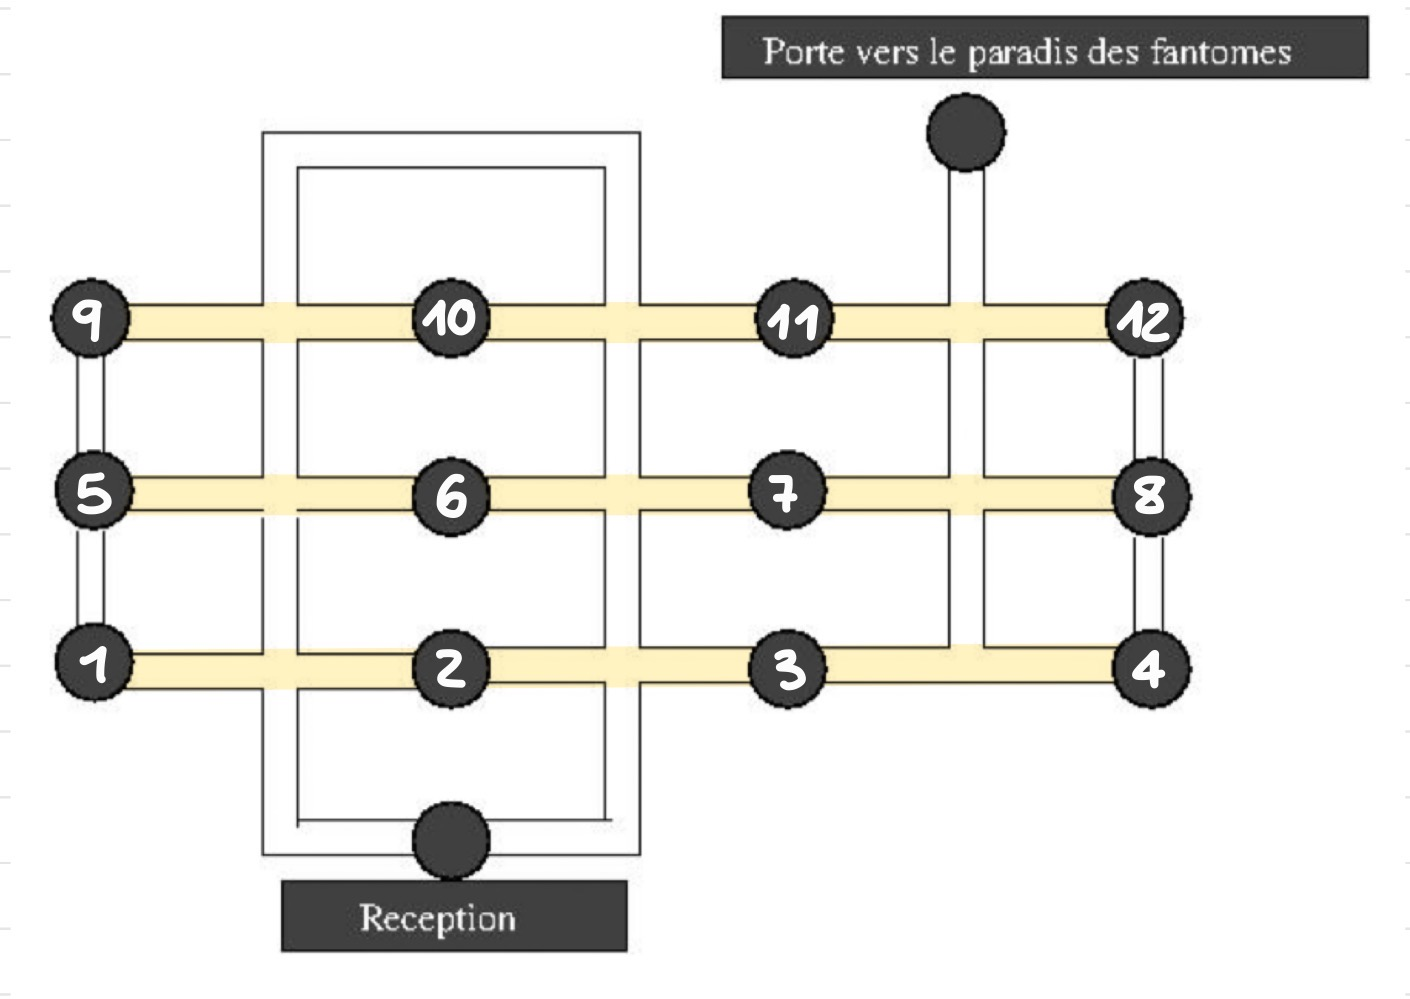
\includegraphics[width=6.5cm]{schema/repetition.JPG} }}%
\end{figure}
\vspace*{2.5cm}
\subsubsection{La fonction Attribution}
\begin{python}
def attribution(fantome, debut,n):
    case_n0 = ' '+str(9-n*4) 
    case_n1 = " "+str(10-n*4)
    """ Attribution de la valeur par defaut des autres cases """
    for i in range(debut,debut+4):
        if fantome == debut :
            case_n0 = colored(' A ', 'magenta', attrs=["blink","bold"])   
        if fantome == (debut+1) :
            case_n1 = colored(' A ', 'magenta', attrs=["blink","bold"])   
        """ Attribution du reste des cases """
    return case_n0, case_n1, case_n2, case_n3
\end{python}
\vspace*{0.5cm}
\hspace*{0.5cm}Cette fonction prend en argument la position du fantôme, le numéro de la case de début et un indice de boucle (pour savoir sur quelle ligne on se trouve). On commence par initialiser les variables avec le numéro de la case en fonction du numéro de la boucle. Ensuite, une boucle parcourra les 4 cases. Pour chaque case de la ligne, on regarde si le fantôme se trouve à l'intérieur, si oui on la modifie pour contenir le pictogramme du fantôme. Sinon, la case contient son numéro propre. Ainsi, on retourne les 4 variables.

\subsubsection{La fonction Print Board}
\begin{python}
def print_board(fantome,pinte):
    """ Affichage de la ligne du paradis """
    for i in range(3):
        if i in [1,2]:
            print(" "*10+"|"+" "*7+"|"+" "*7+"|")
        if i == 0 :
            case_n0, case_n1, case_n2, case_n3 = attribution(fantome,9,i)
        if i == 1 :
            case_n0, case_n1, case_n2, case_n3 = attribution(fantome,5,i)
        if i == 2 :
            case_n0, case_n1, case_n2, case_n3 = attribution(fantome,1,i)    
     """ Affichage de la ligne de la reception et du compteur de pinte """
\end{python}
\vspace*{0.5cm}
\hspace*{0.5cm}La fonction print\_board() prend en arguments la position du fantôme et le nombre de pintes (pour afficher cette information au joueur). Nous avons décidé de placer les lignes du centre du plateau dans une boucle pour factoriser notre code, cependant cela pose deux problèmes majeurs. Tout d'abord, si pour l'affichage du fantôme, si on ne précise pas la ligne sur lequel il se trouve, il finira dans la colonne entière à cause de la boucle. Deuxièmement, afin de faciliter les déplacements du joueur sur le plateau, il nous faut afficher les numéros de cases.\\
\hspace*{0.5cm}Ces deux problèmes sont résolus grâce à la fonction attribution() qui gèrent dynamiquement le contenu des variables à print(). Ce mode de fonctionnement est assez complexe mais il nous permet de très facilement afficher n'importe quelle chose dans les cases sans avoir à modifier de nombreuses lignes de code. Cela fut fort utile au moment ou nous avons décidé d'ajouter de la couleur dais notre programme. 
\vspace*{0.3cm}
\subsection{Déplacement}
\hspace*{0.5cm} Pour ce qui est du déplacement du fantôme, celui ci ne peut qu'aller de pièces en pièces seulement si elles sont reliées par deux couloirs. On remarque qu'on peut visualiser trois différentes zones. Si le fantôme se trouve a gauche il peut aller sur toutes les cases de gauche et celle du centre, si il est à droite, même principe. Ainsi, si il se trouve au centre du plateau il peut se déplacer partout.\\
\begin{figure}[H]%
    \centering
    \subfloat{{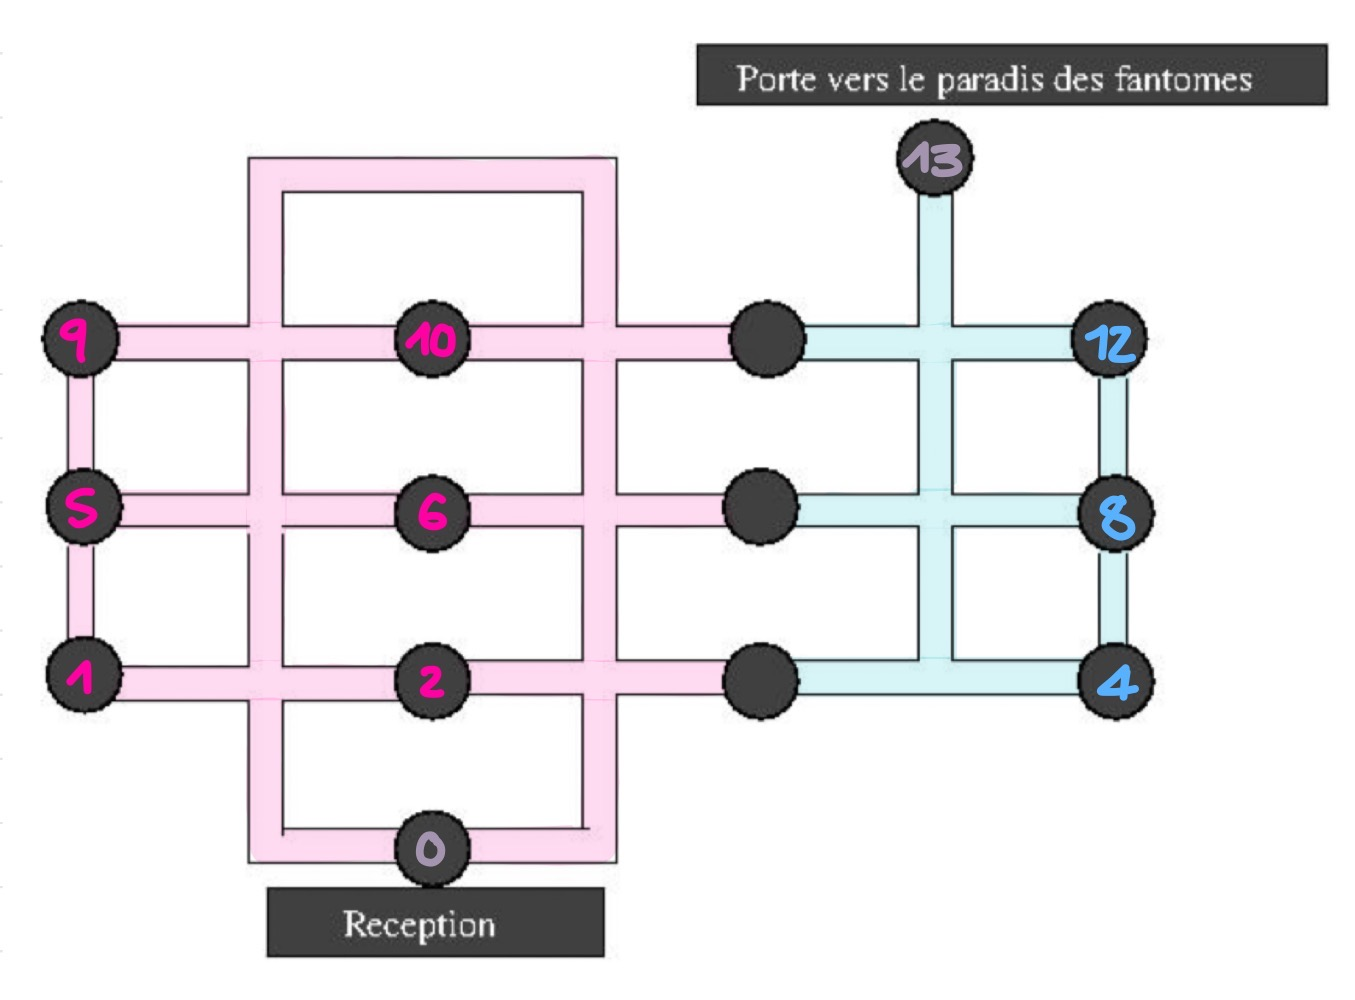
\includegraphics[width=6.5cm]{schema/repartition_1.JPG} }}%
    \qquad
    \subfloat{{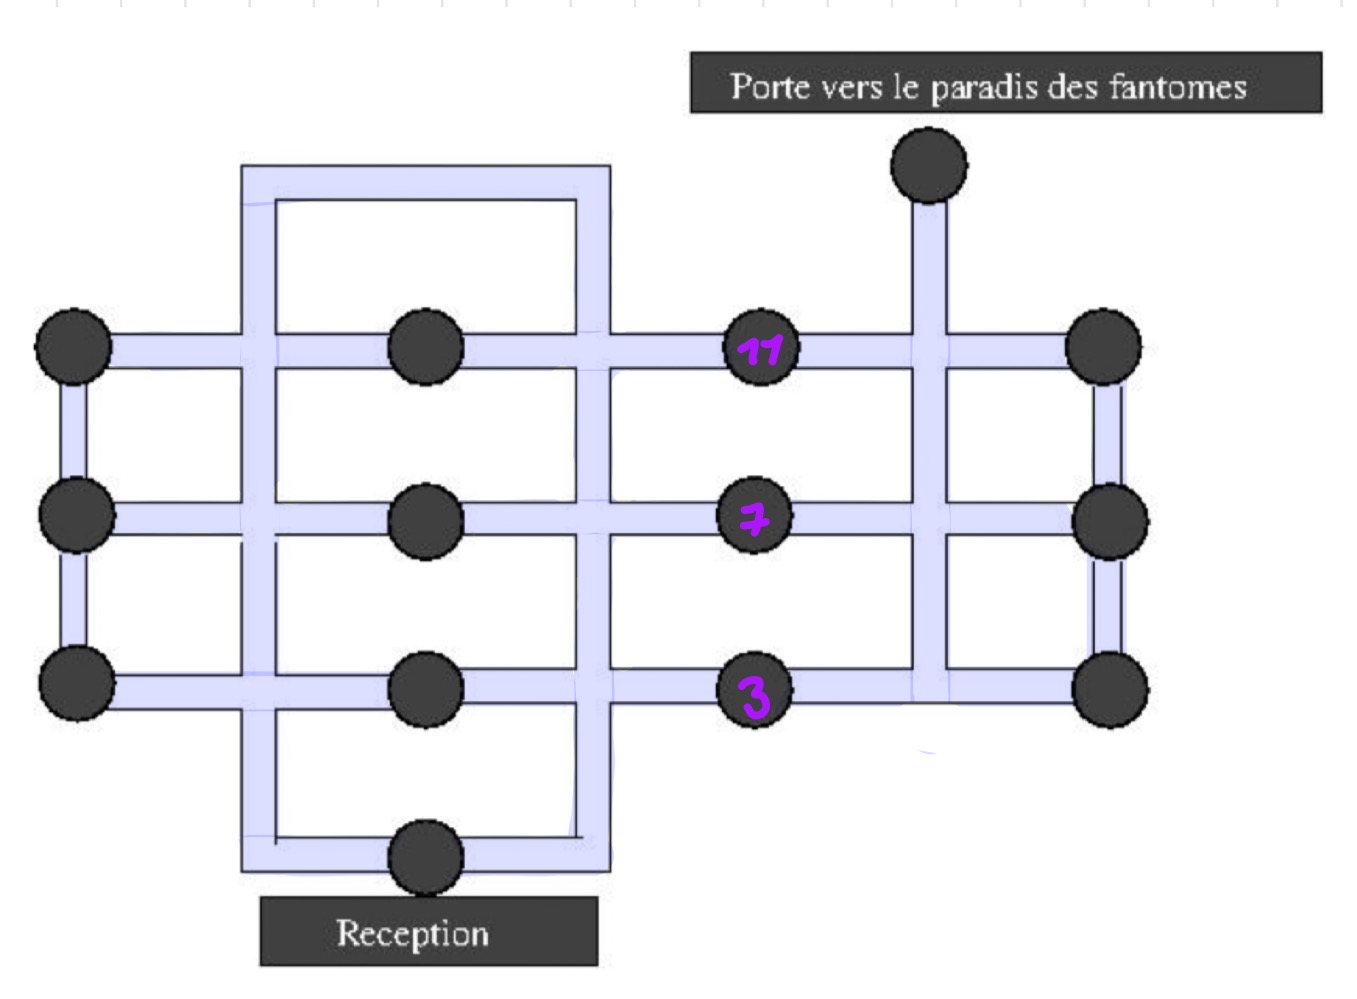
\includegraphics[width=7cm]{schema/repartition_2.JPG} }}%
    \caption{Différente zones accessible au fantômes.}%
    \label{fig:example}%
\end{figure}
\subsubsection{La fonction Is Ok To Move}
\begin{python}
def is_ok_to_move(fantome,wanted_position):
    g1 = [0,1,2,3,5,6,7,9,10,11]
    g2 = [3,4,7,8,11,12,13]
    if wanted_position in [11,7,3]:
        return True
    if fantome in g1 and wanted_position in g1 :
        return True
    if fantome in g2 and wanted_position in g2  :
        return True
    print('Impossible de ce deplacer ici !')
    return False
\end{python}
\vspace*{0.5cm}
\hspace*{0.5cm}Grâce à cette astuce, on peut facilement regarder si le fantôme a le droit de se déplacer avec simplement sa positon et la position de la case voulue. On commence par définir des groupes de cases. Ajouter les cases du centre dans les deux groupes nous permet de faciliter le traitement.\\
\hspace*{0.5cm}Ensuite, on va regarder si la case du fantôme et la case ou il désire aller se trouvent dans le même groupe. Si oui, on retourne True, sinon, on retourne False. Il est bon de noter que si le fantôme se trouve dans une des cases du centre, on retourne directement True sans se poser de questions. 

\subsection{Ennemis}
\hspace*{0.5cm} La conception des ennemis dans le code se fait en 2 parties, d'abord leurs placements et ensuite la relation topographique entre le fantôme et les ennemies.\\
\hspace*{0.5cm}Comme expliqué précédemment dans l'analyse du sujet, on a procédé en 2 étapes. D'abord avec des méchants fixe et ensuite avec une version aléatoire.\\

\begin{figure}[H]%
    \centering
    \subfloat[\centering Schema des ennemis fixes ]{{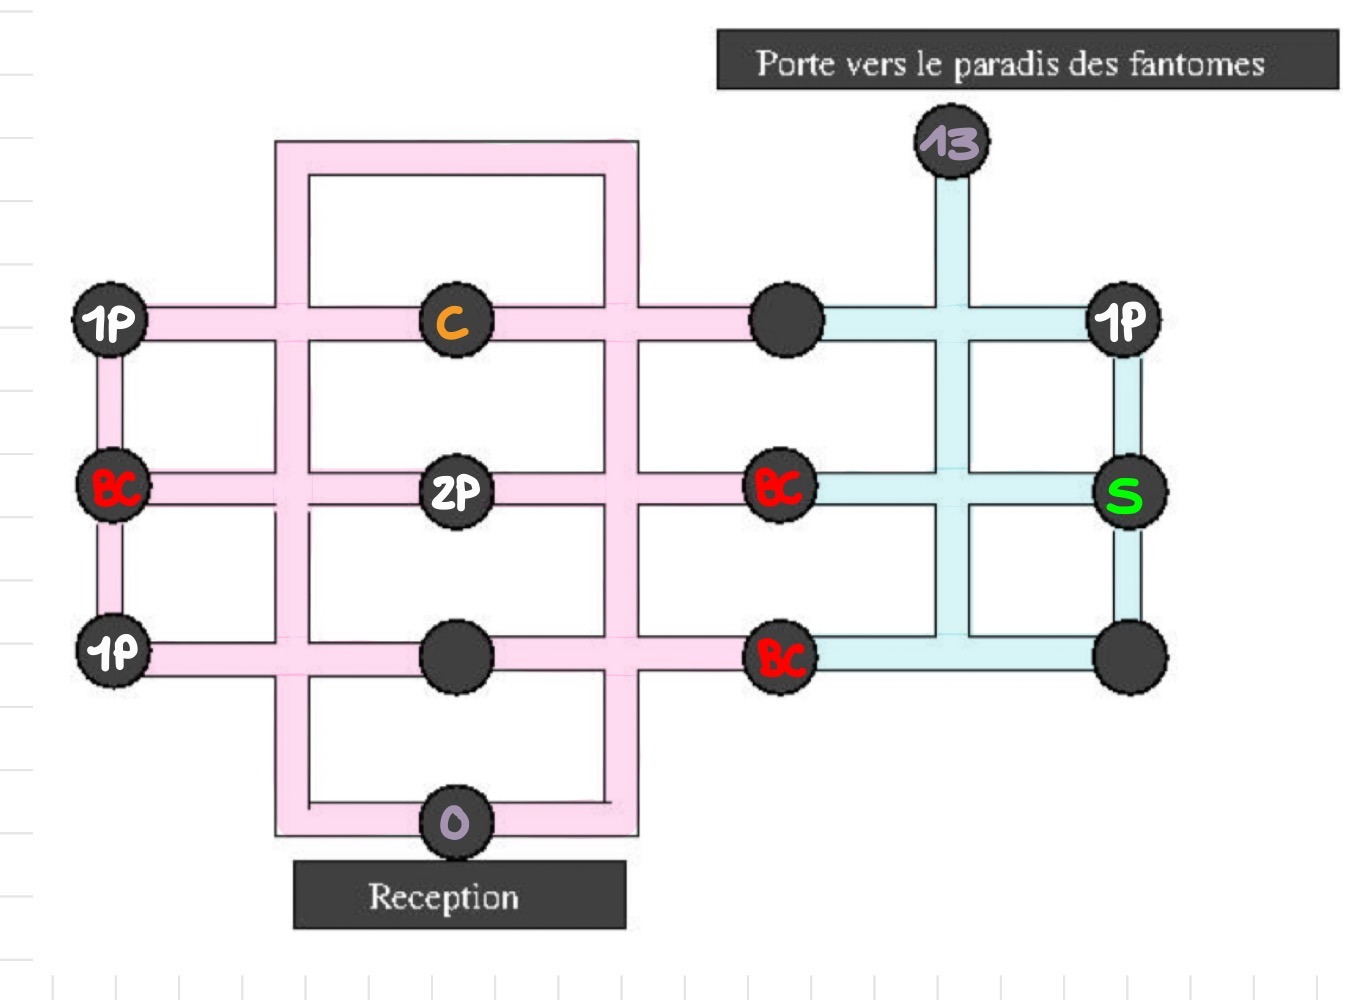
\includegraphics[width=6.5cm]{schema/ennemis.JPG} }}%
\end{figure}

\hspace*{0.5cm}Vous pouvez observer sur le schéma ci-dessus les positions fixes que nous avons choisies. Nous avons délibérément décidé de placer deux des trois bibumdums sur la ligne centrale qui donne accès à toutes les salles, afin de rendre le jeu plus difficile pour le joueur. De plus, nous avons décidé de mettre deux pintes dans une même case dans le but de pousser notre code au maximum, en testant les cas de figure saugrenus. Le reste des positions, sans signification particulière, ont été choisi simplement par préférence personnelle. \\
Afin d'obtenir les réactions aux ennemis souhaitées, nous avons choisi de vérifier si la position des fantômes était la même que celle des ennemis, si oui un message approprié est renvoyé.\\
\subsubsection{La fonction Initialisation des Positions}
\begin{python}
def initialisation_des_positions(alea):
    list_position = [8,10,3,5,7,1,6,6,9,12]
    if alea.upper() == '2':
        list_position = random.sample(range(1,13),10)
    return {"savant":list_position[0],"maitre":list_position[1],
    "bc":list_position[2:5],"pinte":list_position[5:]}
\end{python}
\vspace*{0.5cm}
\hspace*{0.5cm} Chaque position des ennemis est stockée dans un dictionnaire créé par la fonction initialisation\_des\_positions(alea). Cette fonction prend en argument un nombre, 1 ou 2, qui correspond au niveau choisi par le joueur. Elle crée ensuite un dictionnaire avec soit des positions fixes, conservées dans une liste, ou des positions aléatoires entre 1 et 13.\\
\hspace*{0.5cm}C'est donc dans ce dictionnaire que nous puisons la position des méchants et la comparons avec la position actuelle du fantôme afin de déterminer s'il est en danger.\\
\hspace*{0.5cm}Lorsqu'il a fallu faire l'implémentation dans le menu final, nous avions initialement disposé les fonctions dans cet ordre : maître du jeu, bibemdum, et enfin savant, ce qui était une erreur. Il était important de placer la fonction du savant avant toutes les autres, afin de pouvoir ensuite vérifier s'il y avait un ennemi dans la case où celui-ci nous a transportés.\\ 
\subsubsection{La fonction Bruit}
\hspace*{0.5cm} Ensuite, il fallait pouvoir détecter la position des ennemis et renvoyer les messages si le fantôme se trouvait près de l'un d'eux.\\
\hspace*{0.5cm}Pour cette fonction, deux approches se sont présentées : la première consistait à créer une liste pour chaque case, détaillant les voisins possibles de celle-ci. La seconde, se focalisait sur la position de chaque ennemi et impliquait un calcul par rapport à celle-ci.\\
\hspace*{0.5cmNous avons choisi la deuxième option car elle était plus optimisée et que nous avions comme objectif futur d'agrandir le plateau de jeu, ce qui aurait nécessité l'ajout de cases supplémentaires.\\
<\begin{python}
def bruit(fantome, savant, maitre, bc):
    vectors = [-1,1,-4,4,-5,5-3,3]
    savant_pos = [pos+savant for pos in vectors] 
    maitre_pos = [pos+maitre for pos in vectors]
    bc_pos = []
    for i in range(len(bc)): 
        bc_pos.append([pos+bc[i] for pos in vectors])
    print("-"*53)
    if fantome in bc_pos : 
        print("          Vous sentez une odeur de marchmallo")
    if fantome in savant_pos : 
        print("  Vous entendez le rire sardonique du savant fou   ")
    if fantome in maitre_pos : 
        print("Vous entendez les cles du trousseau du maitre du jeu")
    print("-"*53)
\end{python}
\hspace*{0.5cm}Pour cela on a fait la fonction bruit(fantôme, savant, maître, bc), qui prend en entrée les positions de chaque ennemi et qui crée une liste avec toute position possible autour de celui-ci. Si le fantôme ce trouve a une case d'un ennemis, un message approprié s'affiche.\\
\hspace*{0.5cm}La création des listes par rapport au position de chaque ennemi est complexe, c'est pourquoi on a fait un schéma récapitulatif.\\
\begin{figure}[H]%
    \centering
    \subfloat{{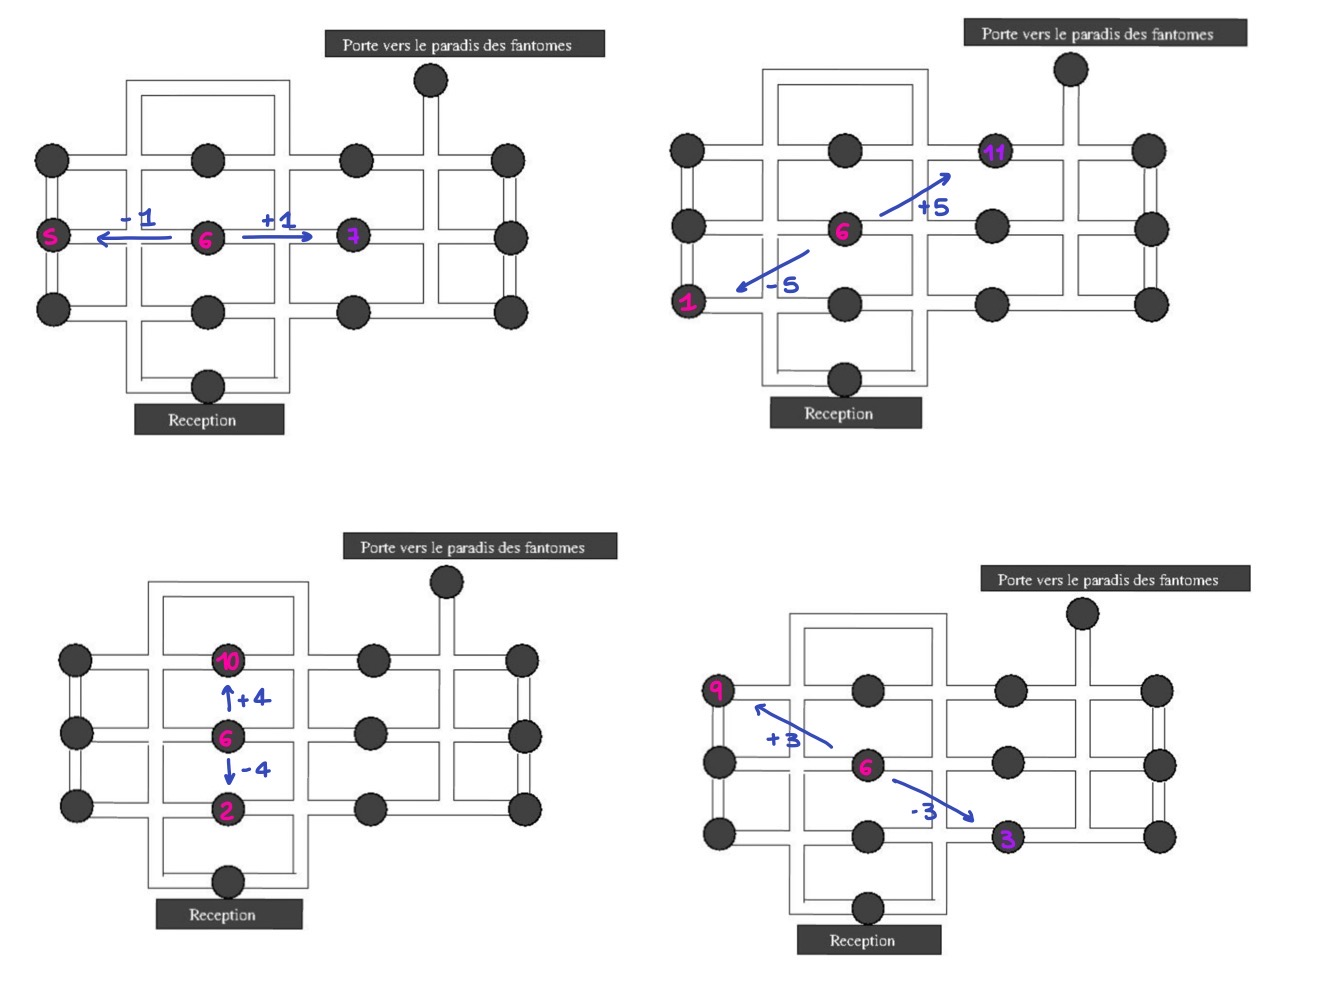
\includegraphics[width=6.5cm]{schema/voisins_1.JPG} }}%
    \qquad
    \subfloat{{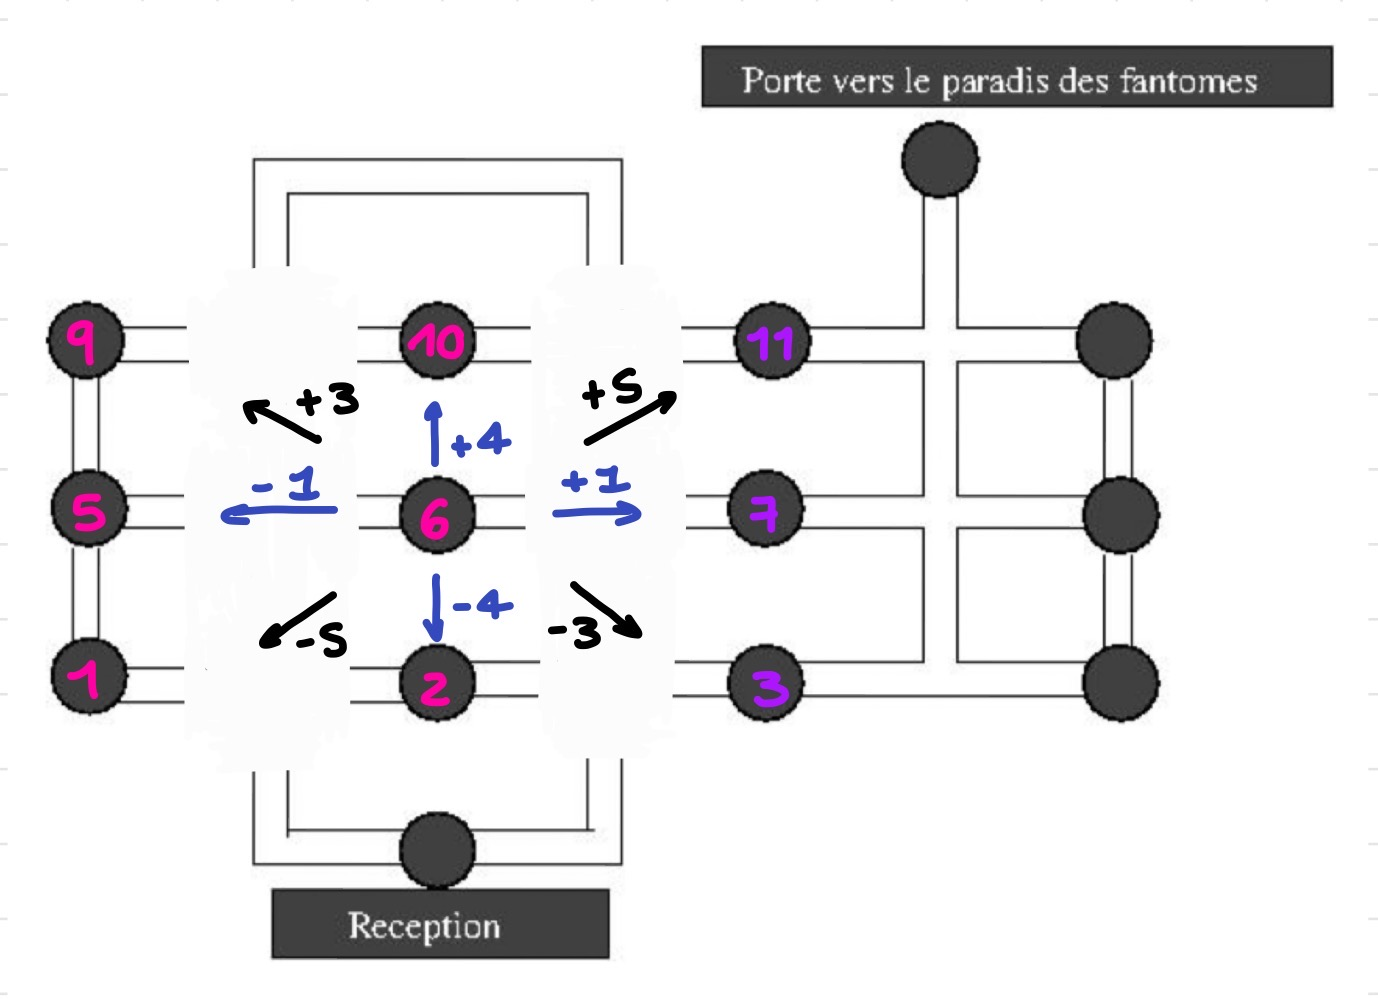
\includegraphics[width=7cm]{schema/voisin_2.JPG} }}%
    \caption{On calcule ces listes grâce a cette structure que vous voyez sur ces schémas}%
    \label{fig:example}%
\end{figure}
\hspace*{0.5cm}Sur ce schéma, on choisit la case 6 comme exemple, les voisins à droite et à gauche son facile, il suffit d'ajouter ou d'enlever 1 pour aller au dessus ou en dessous c'est 4, et pour les diagonales 3 ou 5. Ainsi, nous calculons grâce à des vecteurs toutes les cases avec du bruit de façon dynamique permettant de modifier la position des ennemis sans avoir a re-préciser ces dernières. 

%PARTIE 3
\section{Notre Programme, La Boucle d'Exécution}
\subsection{Déroulé de la partie}

\begin{figure}[H]
    \subfloat[\centering Schéma résumant l'exécution du programme]{{\centering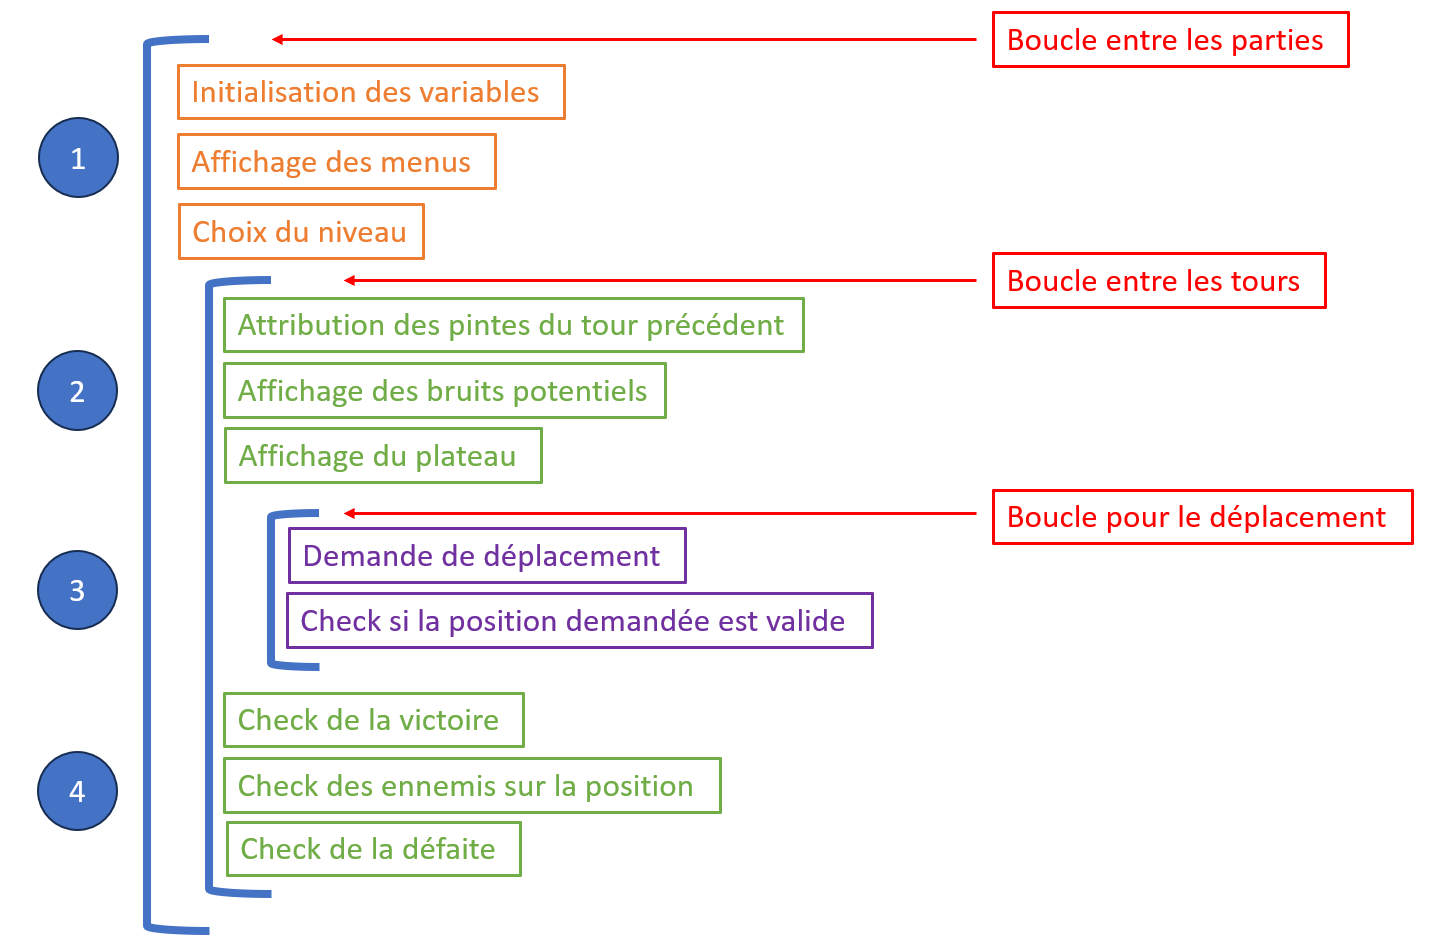
\includegraphics[width=14cm]{schema/programme_principal.png} }}
\end{figure}

\hspace*{0.5cm} Comme mentionné précédemment, notre programme utilise trois boucles pour son exécution, toutes formulées avec "while True". Cette approche permet de relancer le jeu en boucle et assure que l'utilisateur réponde de manière adéquate.

\subsubsection{Début de la boucle principale (1)}
\begin{python}
while True :
    pinte = 2
    casper_position = 0    
    tour = 1 
    menu(affichage_menu()) 
    alea = input("Choix de la difficulte :Lv (1) (2))")
    dico_positions=initialisation_des_positions(alea)
\end{python}
\vspace*{0.5cm}
\hspace*{0.5cm}Cette boucle commence tout d'abord par initialiser les variables de base de la partie. Par exemple, elle initialise le nombre de pintes à 2 et la position du fantôme à 0. Comme cela, en début de partie ou après une partie, les conditions initiales sont restaurées.\\
\hspace*{0.5cm}Dans un second temps, la boucle prend en charge un menu grâce aux fonctions imbriquées menu(affichage\_menu)). En effet, affichage\_menu() retourne le nombre donné par l'utilisateur, et la fonction menu() se charge de présenter le résultat.\\
\hspace*{0.5cm}Finalement, avant de débuter une partie, la fonction initialisation\_des\_positions() est appelée pour placer dans un dictionnaire la localisation des ennemis et des pintes. Cette dernière peut prendre la variable "alea" comme argument pour transformer le dictionnaire de façon aléatoire.\\  

\subsubsection{Début de la partie (2)}
\begin{python}
    while True :
        tour += nouveau_tour(tour)
        pinte += compteur_pinte(dico_positions["pinte"], casper_position) 
        bruit(casper_position, dico_positions["savant"],
            dico_positions["maitre"], dico_positions["bc"]) 
        print_board(casper_position,pinte)
\end{python}
\vspace*{0.5cm}
\hspace*{0.5cm}La partie commence, on appelle la petite fonction tour() uniquement cosmétique qui incrémente de 1 et nettoie le terminal. Ensuite, il est important de calculer le nombre de pintes que possède le joueur au début du tour grâce à la fonction compteur\_pinte(). 
\hspace*{0.5cm}Ensuite, la fonction bruit() décrite plus tôt et appelée et va renseigner le joueur sur les ennemis qui sont proches de lui. Enfin, grâce à la fonction print\_board(), on peut afficher le plateau à la position du joueur. 

\subsubsection{Boucle de déplacement (3)}
\begin{python}
        while True :
            asked_position = int(ask_where_to_go())
            if asked_position == 0 : #Check de demande d'exit
                sys.exit()
            if  is_ok_to_move(casper_position,asked_position):
                casper_position = asked_position
                break
\end{python}
\vspace*{0.5cm}
\hspace*{0.5cm}Dans cette boucle, on veut être sur que le joueur indique une position valable pour son déplacement. Ainsi, on demande au joueur ou il désire aller. Si le joueur donne 0 le programme se termine. En revanche, si il donne un chiffre la fonction is\_ok\_to\_move() est appelée. Elle va retourner False si le joueur n'a pas le droit d'aller à cet emplacement et, la boucle recommence donc pour appeler à nouveau le joueur à entrer un nombre. Si finalement la position est valide, is\_ok\_to\_move() retourne true et la boucle est brisée. 

\subsubsection{Fin du tour (3)}
\begin{python}
        if victoire(casper_position): #Check de   victoire 
            break
        r_value = savant_jeu(casper_position,dico_positions["savant"])
        casper_position = r_value[0]
        pinte += r_value[1]
        casper_position = maitre_du_jeu(casper_position,dico_positions["maitre"]) 
        pinte += bib_jeu(casper_position,dico_positions["bc"])
        if perdu(pinte):
            break
\end{python}
\vspace*{0.5cm}
\hspace*{0.5cm}La fin du programme n'est pas des moindres, on commence par regarder si le joueur s'est déplacé dans la case du paradis ce qui lui donnerait la victoire grâce à la fonction victoire(). Si elle ne retourne rien, on continue.\\
\hspace*{0.5cm}Il est maintenant temps de faire intervenir les différents ennemis. Le Savant va téléporter le joueur dans une case aléatoire sauf le départ et l'arrivée tout en diminuant les pintes de 1. Le Maître du Jeu va renvoyer le fantôme à la case départ en modifiant la position du de ce dernier directement. Finalement, les Bibendums vont enlever deux pintes au joueur. \\
\hspace*{0.5cm}Après que tous les méchants aient joués, on peut regarder si le joueur possède assez de vie. Sinon on affiche l'écran de défaite et on casse la boucle.\\

\subsection{Éléments graphiques}
\subsubsection{Le package Termcolor}
\begin{figure}[H]
\begin{center}
    \subfloat[Exemple d'affichage du plateau coloré]{{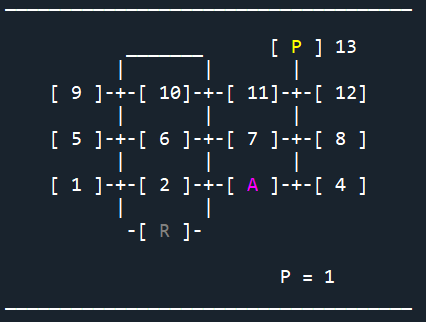
\includegraphics[width=8cm]{schema/color_board.png} }}
    \end{center}
\end{figure}
\hspace*{0.5cm}Notre script gère les affichages en couleur grâce au package Termcolor, ce dernier est compatible avec tous les terminaux classiques et permet diverses options de customisation. Ainsi, notre fantôme est magenta et clignote pour faciliter la lecture du jeu. Ci dessous, un exemple de l'utilisation du package pour obtenir un fantôme coloré :\\ 
\begin{python}
case_n0 = colored(' A ', 'magenta', attrs=["blink","bold"]) 
\end{python}
\subsubsection{La fonction Create a Print}
\begin{python}
def create_a_print(titre, sub , body = ""):
    to_print = ("-"*53+"\n|"+" "*51+"|\n"+titre+"\n"+sub+"\n|"+" "*51+"|\n")
    if body != "" :
        to_print += (body+"\n|"+" "*51+"|\n")
    print(to_print+"-"*53)
\end{python}
\vspace*{0.5cm}
\hspace*{0.5cm}En écrivant notre code, nous nous sommes rendu compte que beaucoup de répétitions étaient présentent dans les affichages des différents événements que le joueur rencontre. A chaque print(), seulement le noms des ennemis et la description du malus changeaient. Ainsi nous avons re-factorisé cet affichage dans la fonction create\_a\_print(). Elle prend comme argument le titre, le sous titre et le corps de texte, elle affiche un menu stylisé et mis en forme avec les différentes conditions.\\
\hspace*{0.5cm}Grâce à cette fonction, nous avons pu modifier notre affichage en cours de route sans avoir à modifier tout notre code. Cela nous a fait gagner beaucoup de temps. 

\section{Perspective d'amélioration}
\hspace*{0.5cm}Bien que notre jeu soit complètement utilisable, il serait pertinent d'ajouter d'autres niveaux pour permettre à l'utilisateur de poursuivre son expérience. En effet, notre code rendrait un tel ajout relativement aisé. Comme notre affichage et nos fonctions sont complètement dynamiques, peu de travail serait nécessaire. 

\section{Conclusion}
Pour conclure ce travail. Voici une liste non exhaustive de ce que nous avons appris à faire lors de cet exercice. Tout d'abord, nous avons pu bien nous organiser et travailler en équipe grâce à la création d'un plan au début de notre projet.D'autre part nous avons aussi appris à utiliser des outils comme GitHub et overleaf pour faciliter le transfert de nos travaux. Finalement, nous avons appris à produire un code complexe dans sa mise en place mais simple dans son utilisation. 

\begin{center}
   \href{https://github.com/Lucien-Piat/Casper}{Enfin, voici la page GitHub du projet }
   \qrcode[height=1cm]{https://github.com/Lucien-Piat/Casper}
\end{center}


\end{document}